%!TEX program = xelatex

\documentclass[openany]{progbookcn}
\usepackage{wrapfig}
\usepackage{enumerate}
\usepackage{amsmath,mathrsfs,amsfonts}
\usepackage{tabularx}
\usepackage{booktabs}
\usepackage{colortbl}
\usepackage{multirow,makecell}
\usepackage{multicol}
\usepackage{ulem} % \uline
\usepackage{listings}
\usepackage{tikz}
\usepackage{tcolorbox}
\usepackage{fontawesome}
\usepackage[open,openlevel=0,atend]{bookmark}
\usepackage{graphicx}
\usepackage{float} 
\usepackage{subfigure}
\usepackage{enumitem}
\usepackage{ctex}

% 用来设置附录中代码的样式

\lstset{
    basicstyle          =   \sffamily,          % 基本代码风格
    keywordstyle        =   \bfseries,          % 关键字风格
    commentstyle        =   \rmfamily\itshape,  % 注释的风格,斜体
    stringstyle         =   \ttfamily,  % 字符串风格
    flexiblecolumns,                % 别问为什么,加上这个
    numbers             =   left,   % 行号的位置在左边
    showspaces          =   false,  % 是否显示空格,显示了有点乱,所以不现实了
    numberstyle         =   \zihao{-5}\ttfamily,    % 行号的样式,小五号,tt等宽字体
    showstringspaces    =   false,
    captionpos          =   t,      % 这段代码的名字所呈现的位置,t指的是top上面
    frame               =   lrtb,   % 显示边框
}

\lstdefinestyle{Python}{
    language        =   Python, % 语言选Python
    basicstyle      =   \zihao{-5}\ttfamily,
    numberstyle     =   \zihao{-5}\ttfamily,
    keywordstyle    =   \color{blue},
    keywordstyle    =   [2] \color{teal},
    stringstyle     =   \color{magenta},
    commentstyle    =   \color{red}\ttfamily,%注释
    breaklines      =   true,   % 自动换行,建议不要写太长的行
    columns         =   fixed,  % 如果不加这一句,字间距就不固定,很丑,必须加
    basewidth       =   0.5em,
}

\setenumerate[1]{itemsep=0pt,partopsep=0pt,parsep=\parskip,topsep=5pt}
\setitemize[1]{itemsep=-1pt,partopsep=0pt,parsep=\parskip,topsep=0pt,itemindent=5pt}
\setdescription{itemsep=0pt,partopsep=0pt,parsep=\parskip,topsep=5pt}
%=========英文字体
\usepackage[osf]{libertinus-otf} 
\usepackage{imakeidx}
\makeindex[%
  intoc=true,
  columns=2,
  columnsep=1cm,
  columnseprule=true
]


\begin{document}

%% title page
\begin{titlepage}
  \vspace*{25ex}

  \hspace{0.05\textwidth}\begin{minipage}{.9\textwidth}
    \flushright

    %%中文书名
    {\zihao{1}\textbf{数学建模竞赛学习笔记}}

    \rule{\linewidth}{.5pt}

    \vspace{2ex}

    %% 副标题
    {\zihao{2}\textsf{从理论到实战}} \\

    \vspace{20ex}

    %% 作者
    {\zihao{4}\textit{谷文军}}
  \end{minipage}

  \vfill

  \centering
  {\zihao{4}镇江 ~$\bullet$ ~ZHENJIANG}
\end{titlepage}
\thispagestyle{empty}


\frontmatter


%% 目录
\clearpage
{
  \hypersetup{hidelinks}
  \tableofcontents
}


\mainmatter

\chapter{初等方法建模}
\section{勾股定理与黄金分割率}
\subsection{黄金分割应用于高跟鞋问题}
\noindent\textbf{原理}:人的下肢长占身高的0.618时,满足最佳黄金比例。\\
\textbf{计算黄金分割最简单的方法}:\\
设某人身高为$h$ cm,下肢长$h_1$ cm,选择高跟鞋的鞋跟高度为$x$ cm,则由建模原理得:
\begin{equation}
{{x+h_1}\over{x+h}}=0.618
\end{equation}
解得:
\begin{equation}
x={{0.618h-h_1}\over 0.382}
\end{equation}
\subsection{黄金分割在其他领域的应用}
\noindent \textbf{医学与0.618的联系}
\begin{itemize}
\item 外界环境温度为人体温度的0.618倍时,人会感到最舒适
\item 养生之道:动与静是一个0.618的比例关系,即四分动六分静是人们认为的最佳养生方式
\item 吃饭六七成饱,几乎不生胃病
\end{itemize}
\noindent \textbf{建筑学与0.618的联系}\\
\noindent \textbf{黄金矩形}

\section{九宫图}
\subsection{九宫图问题的提出}
九宫图又称为三阶幻方,出自西汉(公元前206-公元25)学者戴德编纂的《大戴礼》,源自河图洛书。
\begin{figure}[H]
\centering  %图片全局居中
\subfigure[九宫图]{
\label{Fig.sub.1}
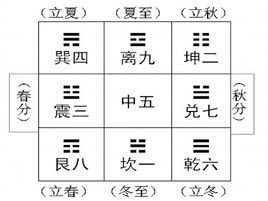
\includegraphics[width=0.3\textwidth]{九宫图}}
\subfigure[河图]{
\label{Fig.sub.2}
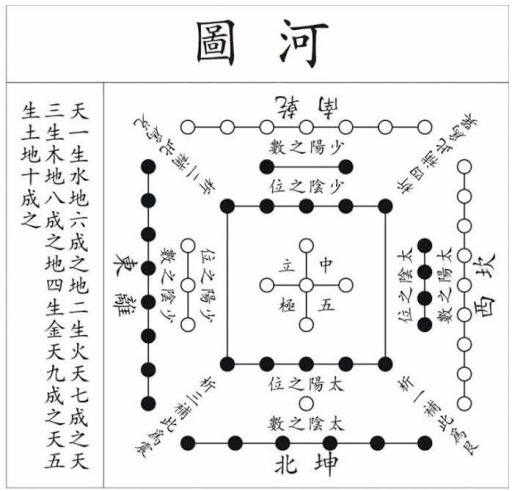
\includegraphics[width=0.3\textwidth]{河图}}
\subfigure[洛书]{
\label{Fig.sub.3}
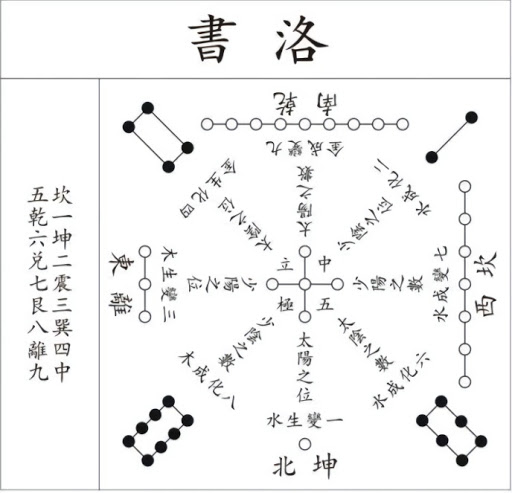
\includegraphics[width=0.3\textwidth]{洛书}}
\caption{九宫图及其起源}
\end{figure}
\indent \textbf{河图}由十种花点组成,分别代表$1-10$这$10$个数,两种花点构成一组,分别布局在东、西、南、北、中五个位置上,每组花点所表示的两个数的差都是$5$。\\
\indent \textbf{洛书}由九种花点组成,分别代表$1-9$这$9$个数,各数的位置排列奇巧,奇偶交替变化,纵横六线及两条对角线上三数之和都为$15$。

\subsection{九宫图问题的求解}
\textbf{口诀一}\\
\indent 九宫者,法以灵龟。二四为肩,六八为足。左三右七,戴九履一,五居中央。\\
\indent \textbf{口诀二}\\
\indent 九子斜列,上下对易,左右相更。四维挺出。
\begin{figure}[H]
\centering
\subfigure[九宫图解一]{
\label{Fig.sub.1}
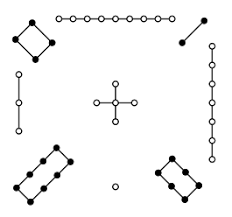
\includegraphics[width=0.2 \textwidth]{九宫图解一}}
\subfigure[九宫图解二]{
\label{Fig.sub.2}
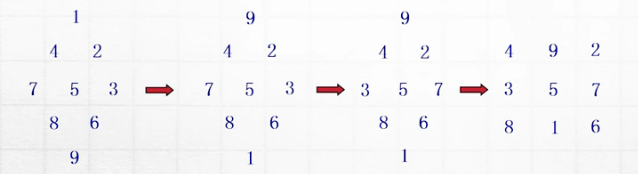
\includegraphics[width=0.6\textwidth]{九宫图解二}}
\caption{九宫图解}
\end{figure}

\section{椅子稳定问题}
\subsection{问题引入与建模准备}
一把四条腿的椅子放在不很平坦的地面上,是否是稳定的?\\
\indent \textbf{不很平坦的定义}:肉眼可见的地面是平坦的\\
\textbf{椅子不稳定的原因}:
\begin{itemize}
\item 椅子的四条腿的长度可能不一样
\item 地面不平坦
\item 椅子的四个底角与地面之间有距离$h,h>0$
\end{itemize}
\indent 三个点确定一个平面,对于相对比较平坦的地面来讲,总可以保证三条腿同时着地,因而只需再使其余的一条腿也能完全着地即可。\\ 
\textbf{量的分析}
\begin{itemize}
\item 椅子的脚和地面的距离作为变量。变量为$0$,意味着椅子的脚与地面没有距离,椅子稳定。
\item 设计旋转角度的连续函数
\end{itemize}

\subsection{模型假设}
\textbf{假设1}:椅子四条腿一样长,椅脚与地面接触处视为一个点,四脚的连线呈正方形$ABCD$,四个椅脚的坐标系中对称;
\begin{figure}[H]
\centering
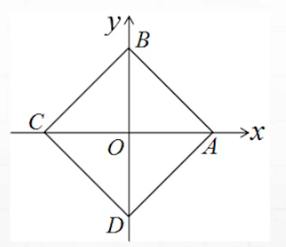
\includegraphics[width=0.3 \textwidth]{figs/chapter3/正方形}
\caption{椅脚坐标系}
\end{figure}

\textbf{假设2}:地面高度使连续变化的,沿任何方向都不会出现间断,如台阶,即地面可视为数学上的连续曲面;\\
\indent \textbf{假设3}:对于椅脚的间距和椅腿长度而言,地面时相对平坦的,使椅子在任何位置至少有三只脚同时着地。


\subsection{模型建立}
\textbf{构造表示距离的函数}:
\begin{itemize}
\item 设$f(\theta)$是$A$、$C$两椅脚与地面的距离之和
\item $g(\theta)$是$B$、$D$两椅脚与地面的距离之和
\item $\theta$是椅子绕中心点$O$旋转角度
\end{itemize}
\begin{figure}[H]
\centering
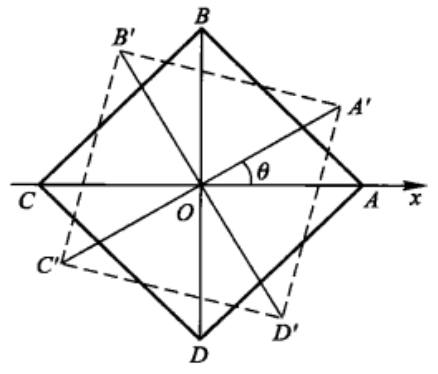
\includegraphics[width=0.3 \textwidth]{figs/chapter3/正方形旋转}
\caption{椅脚坐标系}
\end{figure}
\begin{itemize}
\item 由假设2,$f(\theta)$和$g(\theta)$都是连续函数;
\item 由假设3,椅子在任何位置至少有三只脚同时着地,即对任意的$\theta$,$f(\theta)$和$g(\theta)$中至少有一个为零函数。
\item 在椅子处于初始不稳定的位置时,即$t=0$时,不妨设$g(0)=0,f(0)>0$。
\end{itemize}

\textbf{椅子在不很平坦地面上稳定问题的数学命题}:\\
\indent 已知$f(\theta)$和$g(\theta)$是$t$的连续函数,对任意$\theta$,满足条件$f(\theta) \cdot g(\theta)=0$,且$g(0)=0,f(0)>0$,则至少存在一个$\theta_0$,使$f(\theta_0)=g(\theta_0)=0$,即在旋转椅子的时候,可能在多个位置上都是稳定的。

\subsection{模型求解}
\noindent \textbf{证明}:\\
\indent 将椅子逆时针旋转$\pi\over 2$,则对角线$AC$和$BD$的位置相互交换,且$f(\theta)$和$g(\theta)$是闭区间$[0,{\pi \over 2}]$上的连续函数。\\
\indent 由上面数学命题,一定有下式成立:
\begin{equation}
\begin{cases}
\begin{split}
&g(0)=0,f(0)>0\\
&g({\pi \over 2})>0,f({\pi\over 2})=0
\end{split}
\end{cases}
\end{equation}

\indent 令$h(\theta)=f(\theta)-g(\theta)$,显然$h(\theta)$也是闭区间$[0,{\pi\over 2}]$上的连续函数,\\
\indent 容易检验:$h(\theta)$满足条件$h(0)>0,h({\pi\over 2})<0$。\\
\indent 由闭区间上连续函数的零点存在定理,至少存在$\theta_0$,使得$h(\theta_0)=0$,即$f(\theta_0)=g(\theta_0)$.\\
\indent 再由命题中的条件“对任意$\theta,f(\theta)\cdot g(\theta)=0$”,
得知$f(\theta_0)=g(\theta_0)=0$。

\section{商人过河问题}
\subsection{问题引入}
三个商人各带一名随从渡河,随从们密约:在河的任一岸,一旦随从人数比商人多,就杀人越货。问题:商人该如何设计渡河方案以安全渡河?
\subsection{模型分析}
\noindent \textbf{允许状态集合}\\
\indent $X_k$:第$k$次渡河前此岸的商人数,$X_k,Y_k=0,1,2,3$;\\
\indent $Y_k$:第$k$次渡河前此岸的随从数,$k=1,2,\cdots,n$;\\
\indent 渡河过程的状态:$S_k=(X_k,Y_k)$\\
\indent 允许状态集合:$S=\{(x,y)|x=0,y=0,1,2,3;x=3,y=0,1,2,3;x=y=1,2\}$\\
\textbf{渡河状态集合}\\
\indent $U_k,V_k$:分别任第$k$次渡河船上的商人数与随从数;$(U_k,V_k=0,1,2;k=1,2,\cdots,n)$\\
\indent 决策:$d_k=(U_k,V_k)$\\
\indent 允许决策集合:$D={(u,v)|u+v=1,2}$\\
\textbf {状态转移律}\\
\indent $S_{k+1}=S_k+(-1)^k d_k$
\subsection{模型建立}
制定安全渡河方案归结为如下的多步决策模型:\\
\indent 求$d_k\in D(k=1,2,\cdots,n)$,使$s_k\in S$按状态转移律由$S_1=(3,3)$经有限步$n$到达$S_{n+1}=(0,0)$
\subsection{模型求解}
使用图解法,一共$16$个状态格点,其中允许状态$S$有$10$个点,允许决策$D$表示沿方格移动$1$或$2$格。
\begin{enumerate}[itemindent=2em]
\item [(1).]$k$为奇数,由此岸去彼岸,这时此岸人数减少。移动方向为左/下
\item [(2).]$k$为偶数,由彼岸到此岸,这时此岸人数增多。移动方向为右/上
\item [(3).]$d_k$移动一格表示船上有$1$个人,移动两格表示船上有$2$个人
\item [(4).]用实现表示从此岸去彼岸,虚线表示从彼岸回到此岸
\end{enumerate}
\begin{figure}[H]
\centering
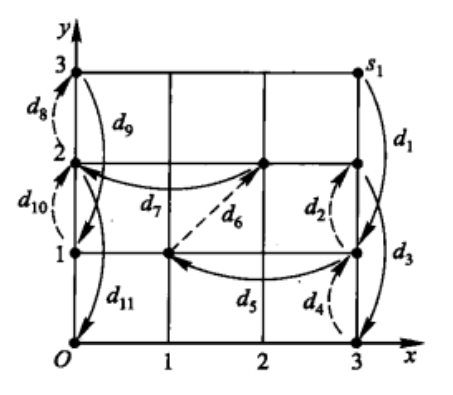
\includegraphics[width=0.45 \textwidth]{figs/chapter3/安全渡河问题图解法}
\caption{安全渡河问题图解法}
\end{figure}


\section{图论方法与网络模型}
\subsection{图论的起源}
图论使组合数学的一个分支,起源于1736年欧拉的第一篇关于图论的论文,这篇论文解决了著名的“哥尼斯堡七桥问题”,从而使欧拉成为图论的创始人。
\subsection{图的概念}
\noindent \textbf{图的定义}\\
\indent 图是一个有序二元组$G={V(G),E(G)}$,其中$V(G)={v_1,v_2,\cdots,v_n}$为顶点集$V(G)$中的元素$v_i$称为顶点,$E(G)={e_1,e_2,\cdots,e_m}$称为边集,$E(G)$中的元素$e_k$叫做边。
\begin{itemize}
\item 顶点总数记位$|V(G)|$,边的总数记位$|E(G)|$
\item 若$|V(G)|=n$,则称$G$为{\bf $n$阶图}
\item 若顶点总数$|V(G)|$与边的总数$|E(G)|$均为有限数,则称$G$为\bf {有限图}
\end{itemize}
\noindent \textbf{有向图的定义}\\
\indent 若顶点集合$V(G)\neq \emptyset$,边集$E(G)\bigcap V(G)=\emptyset$,则称$G=\{V(G),E(G),\emptyset\}$为一个有向图。\\
\noindent \textbf{关联函数}\\
\indent 若$\Phi_G(e)=uv$,$\Phi_G(e)$称为关联函数,表示边$e$与顶点$u$与$v$相关联,又称顶点$u$与$v$相邻,$u$是$e$的尾,$v$是$e$的头,即由$u$指向$v$。\\
\indent 边$e$也成为{\bf 弧},是由两个顶点组成的有序对,通常用尖括号表示。例如:$<v_i,v_j>$,$v_i$称为弧尾,$v_j$称为弧头。$<v_i,v_j>$和$<v_j,v_i>$是两条不同的有向边。\\
\noindent \textbf{无向图的定义}\\
\indent 若$G$的每条边头尾部分,即$\Phi_G(e)=uv=vu$,则称$G$为无向图,无向图中每条边均是顶点的无序对,通常用圆括号表示,例如:$(v_i,v_j)$表示一条无向边,且有$(v_i,v_j)=(v_j,v_i)$。

\subsection{哥尼斯堡七桥问题}
柯尼斯堡七桥问题(Seven Bridges of Königsberg)是图论中的著名问题。这个问题是基于一个现实生活中的事例:当时东普鲁士柯尼斯堡(今日俄罗斯加里宁格勒)市区跨普列戈利亚河两岸,河中心有两个小岛。小岛与河的两岸有七条桥连接。在所有桥都只能走一遍的前提下,如何才能把这个地方所有的桥都走遍?
\begin{figure}[H]
\centering
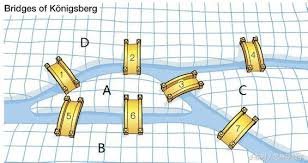
\includegraphics[width=0.6 \textwidth]{figs/chapter3/哥尼斯堡七桥问题}
\caption{哥尼斯堡七桥问题}
\end{figure}
\indent 我们将七桥抽象为无向图中的边,四片陆地抽象为无向图中的点,该无向图可以表示为$G=\{V(G),E(G),\Phi_G\}$,其中$V(G)=\{A,B,C,D\}$,$E(G)=\{a,b,c,d,e,f,g\}$.$\Phi_G(a)=AB$,$\Phi_G(b)=BC$,$\Phi_G(b)=BC$,$\Phi_G(c)=\Phi_G(d)=AC$,$\Phi_G(e)=\Phi_G(f)=AD$,$\Phi_G(g)=BD$。
\begin{figure}[H]
\centering
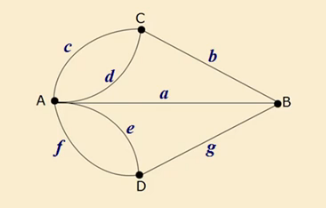
\includegraphics[width=0.6 \textwidth]{figs/chapter3/哥尼斯堡七桥拓扑}
\caption{哥尼斯堡七桥问题图结构}
\end{figure}

\noindent \textbf{七桥问题的图论阐述}\\
\indent 从七桥问题无向图中某个顶点出发,遍历每条边恰好一次,最后能否还回到原来的顶点处(出发点)?


\section{层次分析方法}
\subsection{引子}
\indent 生活中一些问题很难用完全定量的数学模型来解决,对这种复杂决策问题,运用层次分析方法能够找到最佳的解决办法,给出最优的决策。层次分析法(Analytic Hierarchy Process简称AHP)是将与决策有关的元素分解成目标、准则、方案等层次,在此基础上进行定性和定量分析的决策方法。其基本思路与人对一个复杂的决策问题的思维、判断过程大体上是一样的。
\subsection{层次分析法}
\indent 将决策问题按总目标、各层子目标、评价准则直至具体的备选方案的顺序分解为不同的层次结构,然后使用求解判断矩阵特征向量的方法求得每一层次的各元素对上一层次某元素的优先权重,最后再运用加权的方法求出各备选方案对总目标的最终权重向量。其中权重最大者即为最优方案。\\
\indent 层次分析法中每一层的权重设置到最后都会直接或间接影响到结果,而且在每个层次中的每个因素对结果的影响程度都是量化的,非常清晰明确。这种方法擅长于对无结构特性的系统评价以及多目标、多准则、多时期等的系统评价。\\
\indent 层次分析法也具有\textbf{局限性}:
\begin{itemize}
\item 不能为决策提供新方案,层次分析法只能从原有的备选方案中选取最佳方案,因此可能会产生一个由于主观性或者自身创造能力不够而不是最优的方案。
\item 定量数据少,主观因素多,不易令人信服。
\item 指标过多时数据统计量大,且权重难以确定。 当我们希望解决一个具有普适性的问题时,指标的选取数量很可能会随之增加。指标的增加意味着需要构造的层次更深、数量更多、规模更庞大的判断矩阵。
\item 特征值和特征向量的精确求法比较复杂,随着指标的增加,阶数也随之增加,在计算上也变得越来越困难。
\end{itemize}

\subsection{层次分析法的基本步骤}
\noindent 1.{\bf 建立层次结构模型}\\
\indent 在深入分析实际问题的基础上,将有关的各因素按照不同属性自上而下地分解成若干层次,同一层的各个因素因为从属于上一层因素,因此对上层因素会产生较大影响,同时又会支配下一层因素或受到下层因素的影响。\\
\indent 在层次结构模型中,最上层为目标层,通常只有一个因素,最下层通常为方案层,中间可以有一个或几个层次,通常为准则或指标层。当准则过多时(例:$>9$),应进一步分解出子准则层。准则层不宜过少,通常$5-7$个左右。
\begin{figure}[H]
\centering
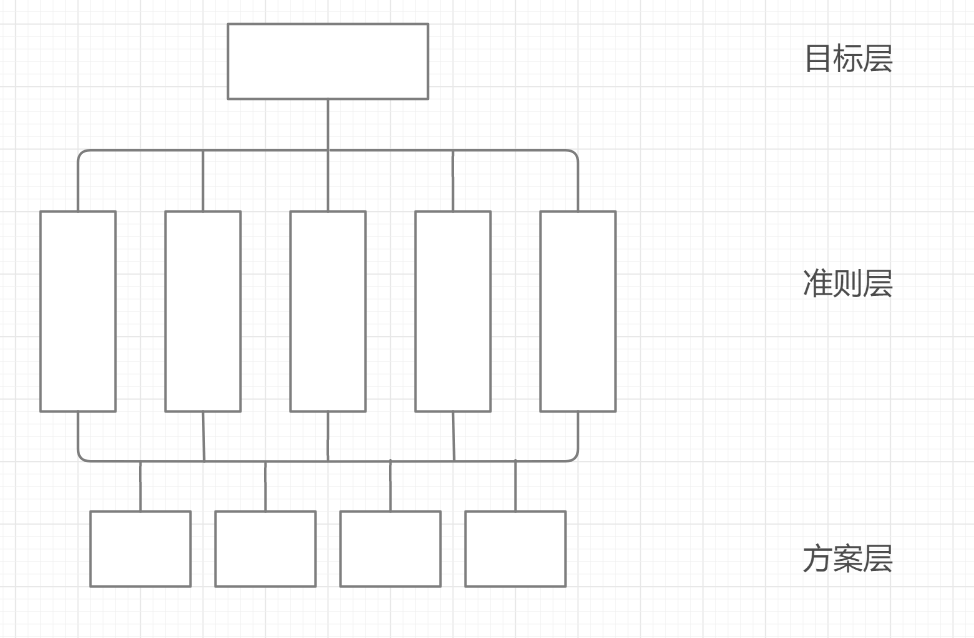
\includegraphics[width=0.6 \textwidth]{figs/chapter3/层次分析结构}
\caption{层次结构模型}
\end{figure}
\noindent 2.{\bf 构造成对比较矩阵}\\
\indent 这一步是要比较层次结构模型的第二层各个因素对上一层因素的影响,从而确定它们对上层因素的影响作用中所占的权重。\\
\indent 设有$n$个因素$x_1,x_2,\cdots,x_n$对上一层目标有影响直接确定它们对目标的影响程度不是很容易,所以每次取两个因素$x_i$与$x_j$比较。用$a_{ij}$表示$x_j$和$x_i$对上层目标的影响比,则$A=(a_{ij})_{m\times n}$称为{\bf 成对比较矩阵},又称为{\bf 正互反矩阵}.
\begin{equation}
A = \left[ {\begin{array}{*{20}{c}}
{\frac{{{x_{\rm{1}}}}}{{{x_1}}}}&{\frac{{{x_1}}}{{{x_2}}}}& \cdots &{\frac{{{x_1}}}{{{x_n}}}}\\
{\frac{{{x_2}}}{{{x_1}}}}&{\frac{{{x_2}}}{{{x_2}}}}& \cdots &{\frac{{{x_2}}}{{{x_n}}}}\\
 \vdots & \vdots & \vdots & \vdots \\
{\frac{{{x_n}}}{{{x_1}}}}&{\frac{{{x_n}}}{{{x_2}}}}& \cdots &{\frac{{{x_n}}}{{{x_n}}}}
\end{array}} \right]_{n\times n},{a_{ij}} > 0,{a_{ii}} = 1,{a_{ij}} = \frac{1}{{{a_{ji}}}}(i = 1,2, \cdots ,n)
\end{equation}
\indent 成对比较矩阵中,每一个$a_{ij}$的取值都是有一定的尺度和规范的,按照Satty的提议,$a_{ij}$在$1-9$及其倒数中间取值。例如:
\begin{itemize}
\item $a_{ij}=1$,元素$i$与元素$j$对上一层次因素的重要性相同
\item $a_{ij}=3$,元素$i$比元素$j$略重要
\item $a_{ij}=5$,元素$i$比元素$j$重要
\item $a_{ij}=7$,元素$i$比元素$j$重要的多
\item $a_{ij}=9$,元素$i$比元素$j$及其重要 
\item $a_{ij}=2,4,6,8$,元素$i$与$j$的重要性介于$1,3,5,7,9$之间
\end{itemize}
\noindent 3.{\bf 计算权向量及一致性检验}\\
\indent 对于每一个成对比较阵计算其最大特征根$\lambda_{max}(A)$及对应特征向量,利用一致性指标、平均随机一致性指标和一致性比率做一致性检验。\\
\indent 若检验通过,那么标准化特征向量即为权向量,若不通过,需要重新构造成对比较阵$A$。\\
\indent 由于成对比较矩阵是我们对复杂事物采取两两比较得到的矩阵,构造过程具有明显的主观性,不可能做到判断具有完全的一致性,难免有误差。所以需要对成对比较矩阵进行一致性检验。\\
\noindent \textbf{定义1}\\
\indent 如果一个正互反矩阵$A$满足$a_{ij}a_{jk}=a_{ik}(i,j,k=1,2,\cdots,n)$则称$A$为一致矩阵,简称一致阵\\
\noindent \textbf{性质1}\\
\indent 如果矩阵$A$是一致阵,那么它的秩为$1$,唯一非零特征根为$n$。\\
\noindent \textbf{性质2}\\
\indent 一致阵的任一列(行)向量都是对应于特征根$n$的特征向量。\\

\noindent \textbf{判别法}\\
\indent 判别一个$n$阶矩阵$A$是否为一致阵,只要计算$A$的最大特征根即可。如果$A$不是一致阵,则可以证明$\lambda_{max}(A)>n$而且$\lambda_{max}(A)>n$越大,说明不一致程度越严重。\\
\noindent \textbf{定义2}\\
\indent 设$\alpha=(\alpha_1,\alpha_2,\cdots,\alpha_n)^T$为正向量,称$\alpha'$为$\alpha$的标准化向量,其中
\begin{equation}
a'=\left( {\frac{{{\alpha_1}}}{{\sum\nolimits_{i = 1}^n {{\alpha_i}} }},\frac{{{\alpha_2}}}{{\sum\nolimits_{i = 1}^n {{\alpha_i}} }}, \cdots ,\frac{{{\alpha_i}}}{{\sum\nolimits_{i = 1}^n {{\alpha_i}} }}} \right)
\end{equation}

\noindent \textbf{一致性检验}\\
设$A$为$n$阶成对比较矩阵
\begin{itemize}
\item {\bf 一致性指标}:$CI={{\lambda-n}\over{n-1}}$来表征一致性程度,当$CI=0$时为一致阵,$CI$越大,$A$的不一致程度越严重。
\item {\bf 平均随机一致性指标}:$RI$来确定$A$的不一致程度的容许范围。对于固定$n$,随机构造成对比较矩阵$A'=(\alpha_{ij}')$其中$a_{ij}'$是从$1,2,\cdots,9$和$1,{1\over 2},\cdots,{1\over 9}$中随机抽取的。这样构造的$A'$是不一致的,它的$CI$相当大。如此构造相当多的$CI$,然后算出这些$A'$的平均值作为平均随机一致性指标的$RI$
\begin{table}[h]
\centering
\caption{随机一致性指标$RI$数值表}
\begin{tabular}{|c|ccccccccccc|}
\hline
{$n$} & $1$ & $2$ & $3$ & $4$ & $5$ & $6$ & $7$ & $8$ & $9$ & $10$ &$11$\\
\hline
{$RI$} & $0$& $0$& $0.58$& $0.90$& $1.12$& $1.24$& $1.32$& $1.41$& $1.45$& $1.49$& $1.51$\\
\hline
\end{tabular}
\end{table}
\item {\bf 一致性比率}:$CR={{CI}\over {RI}}$,当$CR<0.1$时$A$的不一致程度在容许范围内,可用其标准的特征向量$\alpha'$作为权向量,否则需要重新调整判断矩阵$A$
\end{itemize}

\noindent \textbf{权向量的计算方法}
\begin{enumerate}
\item [(1).]如果成对比较矩阵是一致矩阵,则把它的列向量(最大特征根对应的特征向量)标准化得到的向量即为各个因素对上一层目标影响大小的权向量。
\item [(2).]如果成对比较矩阵不是一致矩阵,而它的不一致程度又在容许的范围内,则计算成对比较矩阵的最大特征根及其相对应的特征向量,然后将其标准化,令它作为各个因素对上一层目标影响大小的权向量。
\item [(3).]当成对比较矩阵的不一致程度很严重时,需要重新构造或修正成对比较矩阵。
\end{enumerate}
\noindent \textbf{运用方根法近似计算最大特征值与相应的特征向量}
\begin{enumerate}
\item[(1).] 计算判断矩阵每一行元素的乘积 ${W_i} = \prod\limits_{j = 1}^n {{a_{ij}}(i,j = 1,2, \cdots ,n)}$
\item[(2).]计算$W_i$的$n$次方根${\bar W_i} = \sqrt[n]{{{W_i}}}$
\item[(3).] 对向量${\bar W_i} = ({\bar W_1},{\bar W_2}, \cdots {\bar W_n})$做标准化处理${a_i} = {\bar W_i} \div \sum\limits_{j = 1}^n {{{\bar W}_j}(i = 1,2, \cdots ,n)}$,得到${B=(a_1,a_2,\cdots,a_n)^T}$即为所求的特征向量
\item[(4).] 计算最大特征值${\lambda _{\max }}(A) = \frac{1}{n}\sum\limits_{i = 1}^n {\frac{{{{(AB)}_i}}}{{{a_i}}}}$,其中
\begin{equation}\nonumber
AB{\rm{ = }}\left[ {\begin{array}{*{20}{c}}
{{{(AB)}_1}}\\
{{{(AB)}_2}}\\
 \vdots \\
{{{(AB)}_N}}
\end{array}} \right] = \left[ {\begin{array}{*{20}{c}}
{{a_{{\rm{11}}}}}&{{a_{12}}}& \cdots &{{a_{1n}}}\\
{{a_{21}}}&{{a_{22}}}& \cdots &{{a_{2n}}}\\
 \vdots & \vdots & \vdots & \vdots \\
{{a_{n1}}}&{{a_{n2}}}& \cdots &{{a_{nn}}}
\end{array}} \right] \cdot \left[ {\begin{array}{*{20}{c}}
{{a_1}}\\
{{a_2}}\\
 \vdots \\
{{a_n}}
\end{array}} \right]
\end{equation}
上式中,$(AB)_i$表示向量$AB$的第$i$个元素
\end{enumerate}

\noindent4.{\bf 计算组合权向量并做组合一致性检验}\\
\indent 这是层次分析法的最后一个步骤,需要计算最下层对最上层目标的组合权向量,并做组合一致性检验。若检验通过,则可按照组合权向量表示的结果进行决策,否则需要重新考虑模型或重新构造那些一致性比率较大的成对比较矩阵。
\subsection{假期旅游案例}
\noindent \textbf{问题描述}\\
\indent 假如你在准备一趟假期旅游,有三个景点A、B、C供你选择,你将根据景点费用、居住条件、饮食和旅途等准则比较这三个候选景点,并最终决策选择其中一个景点。\\
\noindent \textbf{层次结构模型}
\begin{figure}[H]
\centering
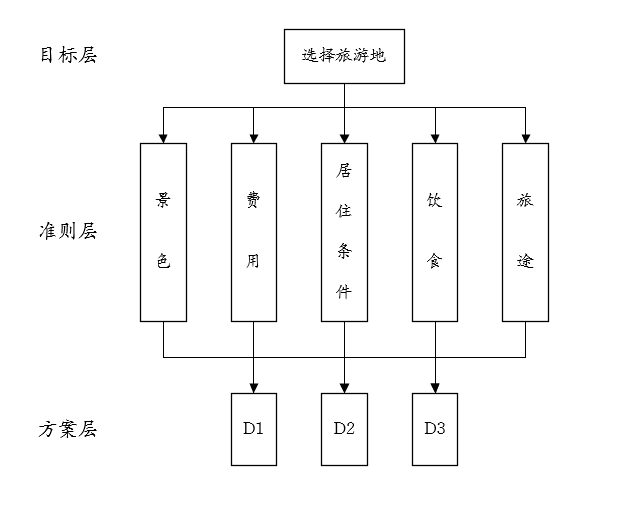
\includegraphics[width=0.6 \textwidth]{figs/chapter3/旅游地选择层次分析模型}
\caption{旅游地选择层次分析模型}
\end{figure}
\noindent \textbf{构造成对比较矩阵}\\
\indent 设景色、费用、居住条件、饮食和交通便利五个因素分别为$X_1$,$X_2$,$X_3$,$X_4$,$X_5$,假设成对比较矩阵如下:
\begin{equation}\nonumber
A = \left[ {\begin{array}{*{20}{c}}
1&{\frac{1}{2}}&4&3&3\\
2&1&7&5&5\\
{\frac{1}{4}}&{\frac{1}{7}}&1&{\frac{1}{2}}&{\frac{1}{3}}\\
{\frac{1}{3}}&{\frac{1}{5}}&2&1&1\\
{\frac{1}{3}}&{\frac{1}{5}}&3&1&1
\end{array}} \right]
\end{equation}
\indent 其中$a_{21}=2$表示费用$X_2$与景色$X_1$对选择旅游地这个目标的比是$2:1$,说明对费用看的更重要一些,其他同理。\\
\noindent \textbf{计算权向量与一致性检验}\\
\indent 运用上一节的方法计算可得最大特征值$\lambda_{max}=5.073$,一致性指标$CI={{\lambda_{max}-n}\over{n-1}}={{5.073-5}\over{5-1}}=0.018$,查表得$RI=1.12$,最终可得一致性比率$CR={{CI}\over{RI}}={0.018\over 1.12}=0.016<0.1$,因此通过了一致性检验。\\
\indent 计算特征根$\lambda_{max}=5.073$对应的特征向量并对其标准化,得$\alpha=\alpha^{(2)}=(0.263,0.475,0.055,0.099,0.110)^T$,为了跟后面得步骤进行区分,这里记位$\alpha^{(2)}$。\\
\indent 从向量中可以看出费用最为重要,其次是景色和旅途,再次是饮食和居住条件。

\noindent \textbf{计算组合权向量并做一致性检验}\\
\indent 三个方案分别针对五个准则构造成对比较矩阵,如下:
\begin{equation}\nonumber
{B_1} = \left[ {\begin{array}{*{20}{c}}
1&2&5\\
{\frac{1}{2}}&1&2\\
{\frac{1}{5}}&{\frac{1}{2}}&1
\end{array}} \right] \quad
{B_2} = \left[ {\begin{array}{*{20}{c}}
1&{\frac{1}{3}}&{\frac{1}{8}}\\
3&1&{\frac{1}{3}}\\
8&3&1
\end{array}} \right] \quad
{B_3} = \left[ {\begin{array}{*{20}{c}}
1&1&3\\
1&1&3\\
{\frac{1}{3}}&{\frac{1}{3}}&1
\end{array}} \right] \quad
{B_4} = \left[ {\begin{array}{*{20}{c}}
1&1&4\\
{\frac{1}{3}}&1&1\\
{\frac{1}{4}}&1&1
\end{array}} \right] \quad
{B_5} = \left[ {\begin{array}{*{20}{c}}
1&1&{\frac{1}{4}}\\
1&1&{\frac{1}{4}}\\
4&4&1
\end{array}} \right]
\end{equation}
\indent $B_1,B_2,B_3,B_4,B5$表示三种旅游方案$D_1,D_2,D_3$分别对准则层中的五个因素(景色、费用、居住条件、饮食和旅途)的影响程度的比较矩阵。例如$B_3$中的$b_{23}=3$表示方案$D_2$与$D_3$相比居住条件好坏的程度之比。\\
\indent 接着分别计算各矩阵的最大特征根以及相应的权向量,再经过标准化得到标准化向量,然后我们还需要对他们分别进行一致性检验,结果如下表:
\begin{table}[h]
\centering
\caption{数值表}
\begin{tabular}{|c|c|c|c|c|c|}
\hline
{$k$} & $1$ & $2$ & $3$ & $4$ & $5$ \\
\hline
{$\alpha_k^{(3)}$}& {$\begin{array}{*{20}{c}}0.595\\ 0.277\\ 0.129\end{array}$} & {$\begin{array}{*{20}{c}}0.082\\0.236\\0.682\end{array}$} & 
{$\begin{array}{*{20}{c}}0.429\\ 0.429\\ 0.142\end{array}$} & {$\begin{array}{*{20}{c}}0.633\\ 0.193\\ 0.175\end{array}$} & {$\begin{array}{*{20}{c}}0.166\\0.166\\0.668\end{array}$}  \\
\hline
{$\lambda_k$}&3.005 &3.002 & 3 & 3.009 & 3\\
\hline
{${CI}_{k}$}&0.003 &0.001 & 0 &0.005 & 0\\
\hline 
{${CR}_k$}&0.052 &0.002 &0 &0.009 & 0 \\
\hline
\end{tabular}
\end{table}
\\
\indent 显然,这5个矩阵都通过了一致性检验,其中$\alpha_k^{(3)}$即为组合权向量,表示第二层对第一层以及第三层对第二层各个因素的综合影响。\\
\indent 最终我们需要的组合权向量$\alpha^{(3)}=\alpha_k^{(3)}\times \alpha^{(2)})=(0.300,0.246,0.456)^T$,即表示三个景点$D_1,D_2,D_3$中分别占的比重,所以可知方案$D_3$占有更高的比重,因此应该选择方案$D_3$。
\section{双层玻璃问题}
\subsection{问题的提出}
\indent 来自北方的同学可能会知道,身边很多的玻璃窗都是双层的,两层玻璃之间是真空的空隙。那么这样的工艺有什么好处呢?它可以有效的阻止室内温度想室外的扩散。那么当建筑物室内外的热传递过程处于热力学平衡状态时,这种构造形式的双层玻璃窗究竟能比单层玻璃窗阻止多少热量损失?两层玻璃窗之间的距离控制在多少为好?
\subsection{量的分析}
\noindent\textbf{符号说明}
\begin{table}[htbp]
\centering
\caption{符号表}
\begin{tabular}{|c|l|}
\hline
符号 & 说明 \\
\hline
{$T_1$} & 室内温度\\
{$T_2$} & 室外温度\\
{$d$} & 单层玻璃温度\\
{$l$} & 两层玻璃之间的空气温度\\
{$T_a$} & 内层玻璃的外侧温度\\
{$T_b$} & 外层玻璃的内测温度\\
{$k$} & 热传导系数\\
{$Q$} &热量损失\\
\hline 
\end{tabular}
\end{table}
\subsection{模型假设}
\begin{enumerate}
\item 热量的传播过程只有传导没有对流,即窗户的密封性能良好,两层玻璃之间的空气是不流动的
\item 室内温度和室外温度保持不变,热传导过程已处于稳定状态即沿热传导方向,单位时间内通过单位面积的热量是常熟
\item 玻璃材料均匀,热传导系数是常数
\begin{figure}[H]
\centering
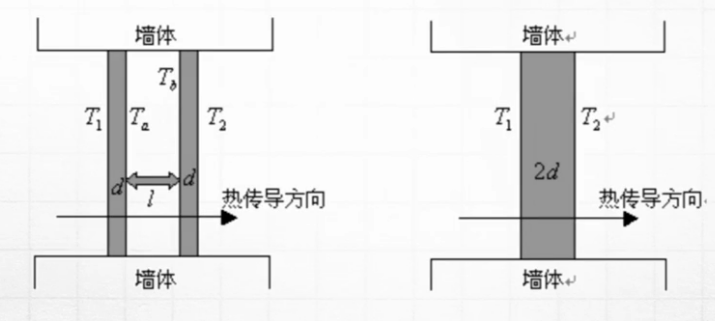
\includegraphics[width=0.6 \textwidth]{figs/chapter3/玻璃热传导示意图}
\caption{玻璃热传导示意图}
\end{figure}
\end{enumerate}
\subsection{模型建立}
\noindent \textbf{热力学传导定律}\\
\indent 厚度为$d$的均匀介质,两侧温度差为$\Delta T$,则单位时间由温度高的一侧向温度低的一侧通过单位面积的热量$Q$与温度差$\Delta T$成正比,与介质的厚度$d$成反比,即
\begin{equation}
Q=k{{\Delta T}\over d}
\end{equation}
\indent 其中,$k$为热传导系数。\\
\noindent \textbf{双层玻璃的热量流失}\\
\indent 由热传导方程遵从的物理定律得知
\begin{equation}
Q=k_1{{T_1-T_a}\over d}=k_2{{T_a-T_b}\over l}=k_1{{T_b-T_2}\over d}
\end{equation}
\indent 由(3.7)式,可知
\begin{equation}
T_1-T_a=T_b-T_2={{dQ}\over k_1},T_a-T_b={{lQ}\over k_2}
\end{equation}
\indent 从而得到
\begin{equation}
T_1-T_2=(T_1-T_a)+(T_a+T_b)+(T_b-T_2)=({{{2d}\over k_1}+{l\over{k_2}}})Q
\end{equation}
\indent 由此可知
\begin{equation}
Q={{k_1(T_1-T_2)}\over{d(s+2)}},s=h{k_1\over k_2},h={l\over d}
\end{equation}

\noindent \textbf{单层玻璃的热量流失}\\
\indent 对于厚度为$2d$的单层玻璃窗户,其热量流失为
\begin{equation}
Q'=k_1{{T_1-T_2}\over{2d}}
\end{equation}
\noindent \textbf{单层玻璃窗和双层玻璃窗热量流失比较}\\
\indent 由$(3.7)$式和$(3.11)$式,可知:
\begin{equation}
{Q\over Q'}={2\over{s+2}}<1
\end{equation}
\indent 因此可见,双层玻璃窗热量流失一定是小于单层玻璃窗的。\\
\indent 已知不流通、干燥空气的热传导系数是$k_2=2.5\times 10^{-4}(J/cm\cdot s\cdot\mbox{度} )$,常用玻璃的热传导系数是$k_1=4\times 10^{-3}-8\times 10^{-3}(J/cm\cdot s\cdot \mbox{度})$,于是${k_1\over k_2}\in[16,32]$。\\
\indent 在分析双层玻璃窗比单层玻璃窗可减少多少热量损失时,我们做最保守的估计,即取$k_1\over k_2$的最小值16,由$(3.7)$式和$(3.11)$式可得:
\begin{equation}
{Q\over Q'}={1\over{8h+1}},h={l\over d}
\end{equation}
\subsection{模型分析与求解}
\indent 比值${Q\over Q'}=(8h+1)^{-1}$反映了双层玻璃窗在减少热量损失的功效,它只与$h={l\over d}$有关。
\begin{figure}[H]
\centering
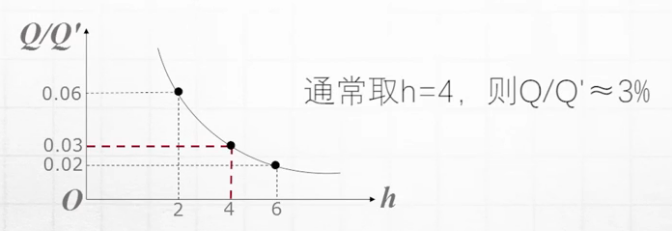
\includegraphics[width=0.6 \textwidth]{figs/chapter3/热量损失比重}
\caption{热量损失比重示意图}
\end{figure}
\indent 通过描述曲线,我们可以观察到$h=4$时,${Q\over Q'}\approx 3\%$,即$Q\approx 3\% Q'$,也就是说双层玻璃窗热量损耗是单层玻璃窗的$3\%$,换句话说双层玻璃窗能够阻止$97\%$的热量,要比单层玻璃窗的功效更好。从图中可以看到,从$h=4$往后,曲线的走势趋于平缓,减少热量损失的功效不明显,因此实际操作时可以建议操作者,双层玻璃窗之间的厚度和玻璃之间的比值控制在$4$倍即可。


\backmatter


\cleardoublepage
%% 索引
\printindex

%% 参考文献
\bibliographystyle{plain}

\end{document}

%%% Local Variables:
%%% mode: latex
%%% TeX-master: t
%%% End:
